 \documentclass[11pt,a4paper]{article}
\usepackage[a4paper,margin=2cm]{geometry}
\usepackage[]{graphicx}
\usepackage{bm}
\usepackage[strings]{underscore}
\usepackage{apacite}
\bibliographystyle{apacite}
\usepackage{svg}
\usepackage{multirow}
\usepackage{amsmath}
\setlength{\parindent}{0pt}
\graphicspath{ {./images} }
\usepackage{wrapfig}
\usepackage{float}
\usepackage[autostyle, english = american]{csquotes}
\usepackage[toc,page]{appendix}
\usepackage{amssymb}
\MakeOuterQuote{"}
\usepackage[T1]{fontenc}
\usepackage{enumitem}
\svgpath{./Diagrams}
\renewcommand{\baselinestretch}{1.1}
\setlist[enumerate]{itemsep=0mm}
\setlist[itemize]{itemsep=0mm}
\begin{document}
\nocite{*}

\begin{titlepage}


\title{Determining the relationship between masses in equilibrium and the angle of a frictionless plane}

\author{Noah Alexiou}


\date{May 2025}

\maketitle
\centering

\end{titlepage}
\tableofcontents
\newpage

\section{Introduction}

\subsection{Research Question}
When the mass of an object on a frictionless plane is altered, and the mass of a hanging object adjusted so equilibrium is achieved, what is the precision and uncertainty of this method in comparison to conventional measuring techniques? 

\subsection{Rationale}

The original experiment was conducted to determine the relationship between the mass of a carriage ($C_m$) and a hanging mass ($H_m$) when a frictionless plane was inclined at different angles. The results confirmed the theoretical relationship $H_m = C_m \sin(\theta)$.

It was noticed during the experiment that the angle measurement device, an `angle gun', had a large uncertainty ($\pm0.5\deg$) compared to the scale used to measure masses ($\pm0.005$ grams). It was questioned whether the relationship between the masses in equilibrium could be used to determine the angle of the plane with improved precision and uncertainty. 
\newline
\begin{figure}[h]
	\centering
	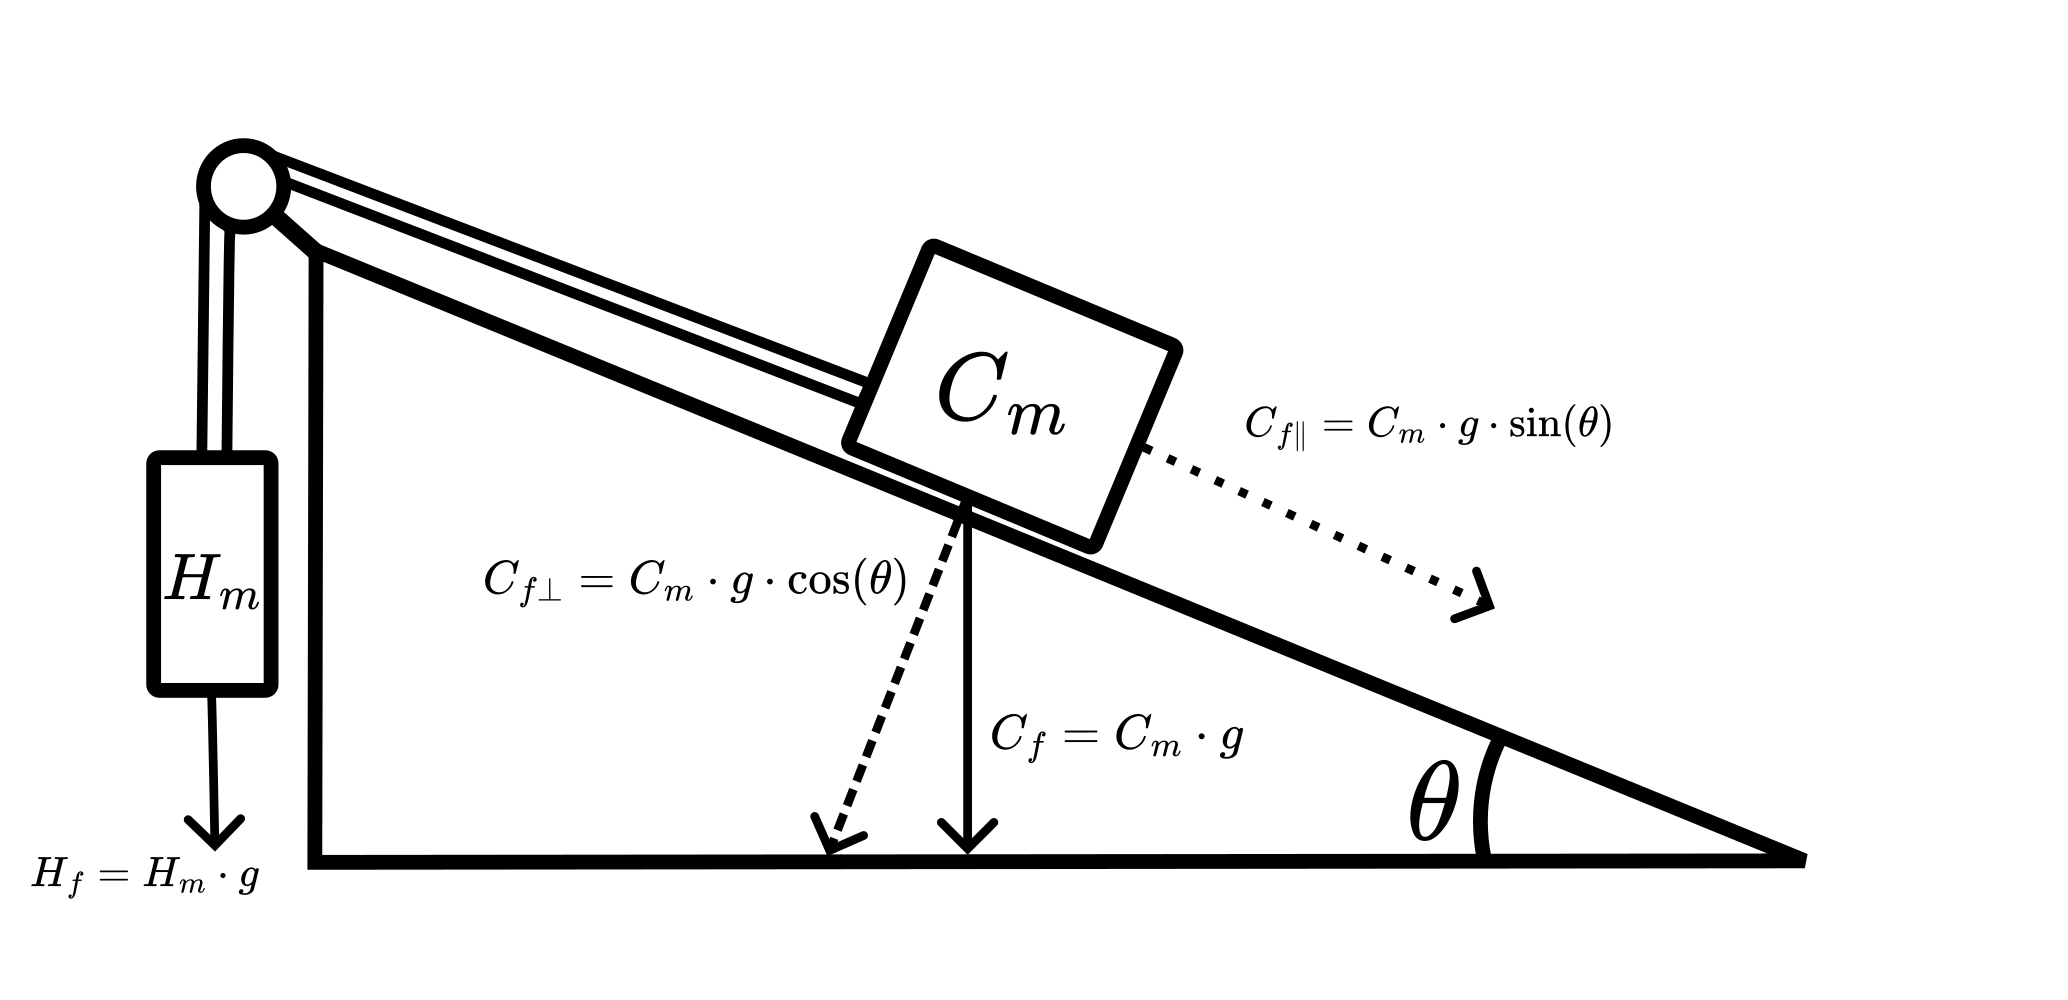
\includegraphics[width=0.5\paperwidth]{./Diagrams/set_upV2.png}
	\caption{Diagram of experimental setup}
\end{figure}
\newline
Considering Newtons first law, under equilibrium the net force is 0 \cite{encyclopediabritannica_2023_newtons}. This implies that under equilibrium,  $C_{f\parallel}=H_f$.

By plotting the experimental results in Excel, a line of best fit can be determined. Since the relationship between the masses is established to be linear, we can use the gradient as a parameter to calculate the angle. 

\begin{center}
	\begin{align*}
	H_m= &\;C_m\cdot{\sin(\theta)} \\
	C_m= &\;H_m\cdot\frac{1}{{\sin(\theta)}}\;\;\;\; \;\;\;\;\;\because \textrm{Make dependent variable subject} \\
	\frac{C_m}{H_m}=&\;\textrm{gradient}	\;\;\;\;\;\;\;\;\;\;\;\;\;\;\because \textrm{gradient}=\frac{\textrm{rise}}{\textrm{run}}\\
\linebreak
	\frac{H_m}{C_m}=&\;\frac{1}{\mathrm{gradient}}=\sin(\theta) \because \sin(\theta)=\frac{O}{H}\\
	\therefore  \;\theta=&\;\sin^{-1}\left(\frac{1}{\textrm{gradient}}\right)
	\end{align*}
\end{center}


Since the angle is now expressed in terms of the gradient, the maximum and minimum slopes derived from experimental data can be used to determine the uncertainty in the angle by calculating the angle using each one of these extremes, then dividing the difference between them by $2$.




\subsection{Methodology}

\subsubsection{Modifications}


The following modifications to the method were implemented
\begin{itemize}
	\item The plane was kept at a constant angle throughout the entire duration of the experiment. This was done to isolate it from the independent and dependent variables and ensure that the results of all trials would point to the same relationship between them and the angle.
	\item The independent variable became the hanging mass ($H_m$). Since this mass could be directly measured and processed without the use of trigonometric functions, the only uncertainty in it's value should be random error from the scale. By conducting multiple trials with the same parameters, random error can be negated. 
	\item The dependent variable became the carriage mass ($C_m$) as the large area inside each carriage allowed for fine adjustment of its mass via the addition of brass weights. 
\end{itemize}

\subsubsection{Materials}
\begin{itemize}
	\item Angle gun 
	\item Measuring tape
	\item Frictionless plane
	\item Pulley
	\item Blower fan
	\item Brass weights
	\item Blue tack 
	\item Scale
	\item Carriage
\end{itemize}

\subsubsection{Method}
\begin{enumerate}
\item Set up slope at a constant angle as shown in Figure 1. It will remain at this angle for the entire duration of the experiment. 
\item Perform and record the following measurements
\begin{itemize}
	\item Along the length of the plane from the ground, to very edge of where the string pivots downwards. Record as "Hypotenuse"
	\item From the point on the ground used as the starting point for the first measurement to the point in which the tensioned string that $H_m$ is connected to touches the ground. Record as "Adjacent"
	\item From the edge of the point where the string pivots downwards to the ground. Record as "Opposite"
	
\end{itemize}
\item Set the hanging mass ($H_m$) to its minimum value initially.
\item Turn on the blower fan
\item Alter the mass of the carriage $(C_m)$ until equilibrium with the $H_m$ is achieved, i.e. The carriage remains stationary. 
\item If the carriage does not have sufficient space for more weight, replace with a larger carriage or link an additional carriage to the chain.  
\item Turn off blower fan
\item Measure and record masses. 
\item Repeat for 3 trials with current $H_m$ value.
\item Increase $H_m$ by 50 grams. 
\item Repeat until $H_m\geq\approx 300$g or until equilibrium cannot be achieved with equipment.
\end{enumerate}


\subsubsection{Risk Assessment}
\begin{table}[h]
	\centering
	\scalebox{0.7}{
		\centering
\begin{tabular}{lllll}
	\textbf{Object}    & \textbf{Risk}                         & \textbf{Effect}               & \textbf{Negation}                          &  \\
	Frictionless plane & Mishandling can cause heavy masses to  & Injury, damage to equipment   & Only turn on blower when required          &  \\
	& travel down the slope at high speeds  &                               &                                            &  \\
	Frictionless plane & Low fan speed causes insufficient air & Friction, damage to equipment & Use maximum fan speed                      &  \\
	& pocket under carriage(s)              &                               &                                            &  \\
	Blower fan         & Overheating                           & Damage to equipment           & Only turn on blower when required          &  \\
	Heavy masses       & Falling on personnel or equipment     & Injury, damage to equipment   & Carefully handle masses, minimise distance &  \\
	&                                       &                               & between scale and experimental setup, wear &  \\
	&                                       &                               & enclosed footwear                          & 
	\end{tabular}
}
\end{table}
\section{Results and Evaluation}
\subsection{Results}

\subsubsection{Raw Data}
\begin{center}
	\centering
	\begin{figure}[h]
		\centering
		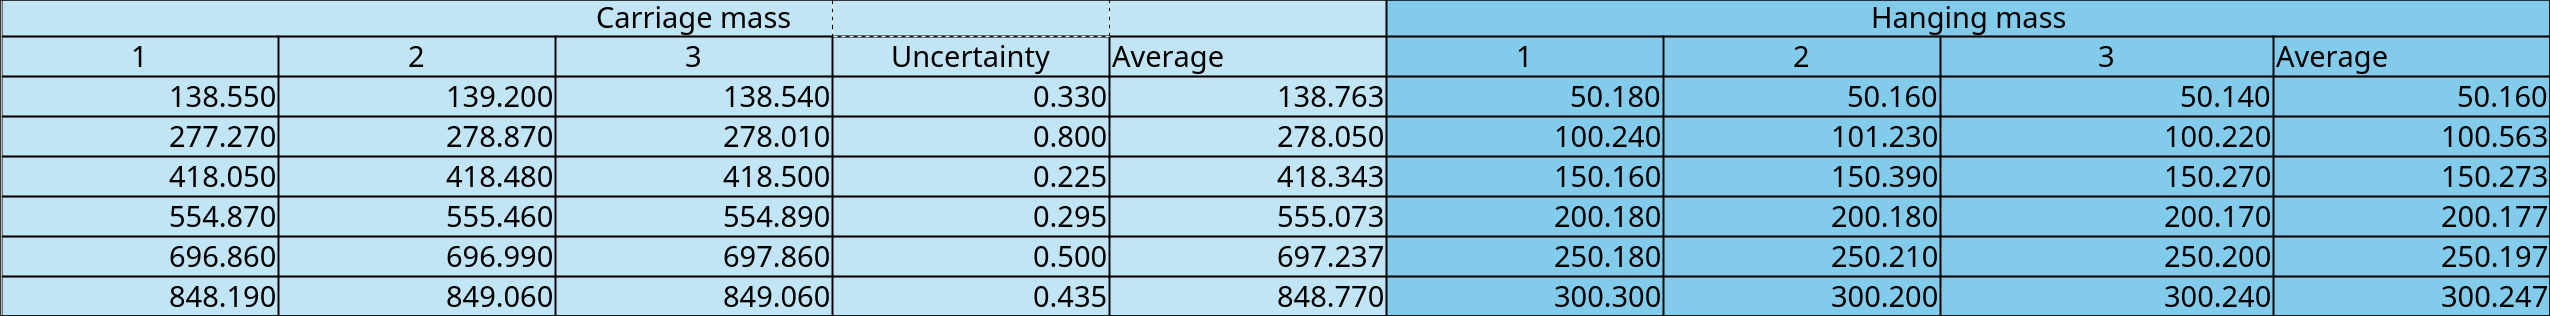
\includegraphics[width=0.84\paperwidth]{resultstable.png}
		\caption{Raw results with additional calculations}
	\end{figure}
	
\end{center}


\subsubsection{Sample Calculations}
\begin{center}
\textbf{Absolute uncertainty for $C_m$ when $H_m=50.160$}
\begin{align*}
	\sigma(C_m)=&\pm\frac{\textrm{max}-\textrm{min}}{2}\\
	=&\pm\frac{139.20-138.55}{2}
	\\=&\pm0.325
\end{align*}
\newline

\textbf{Average mass of $C_m$ when $H_m=50.16$}
\begin{align*}
	\bar{C_m}=&\frac{\Sigma^n_{i=1}C_m}{n}\\
	=&\frac{138.55+139.20+138.54}{3}\\
	=&137.76
\end{align*}
\end{center}


\subsubsection{Prerequisite trigonometric measurements}

\begin{figure}[H]
	\centering

	\begin{tabular}{|l|l|l|}
		\hline
		\textbf{Hypotenuse} & \textbf{Length} & \textbf{Height} \\ \hline
		2.65       & 2.50   & 0.98   \\ \hline
	\end{tabular}

	\caption{Table showing the side lengths of triangle formed by incline plane}
\end{figure}


\begin{figure}[H]
	\centering
	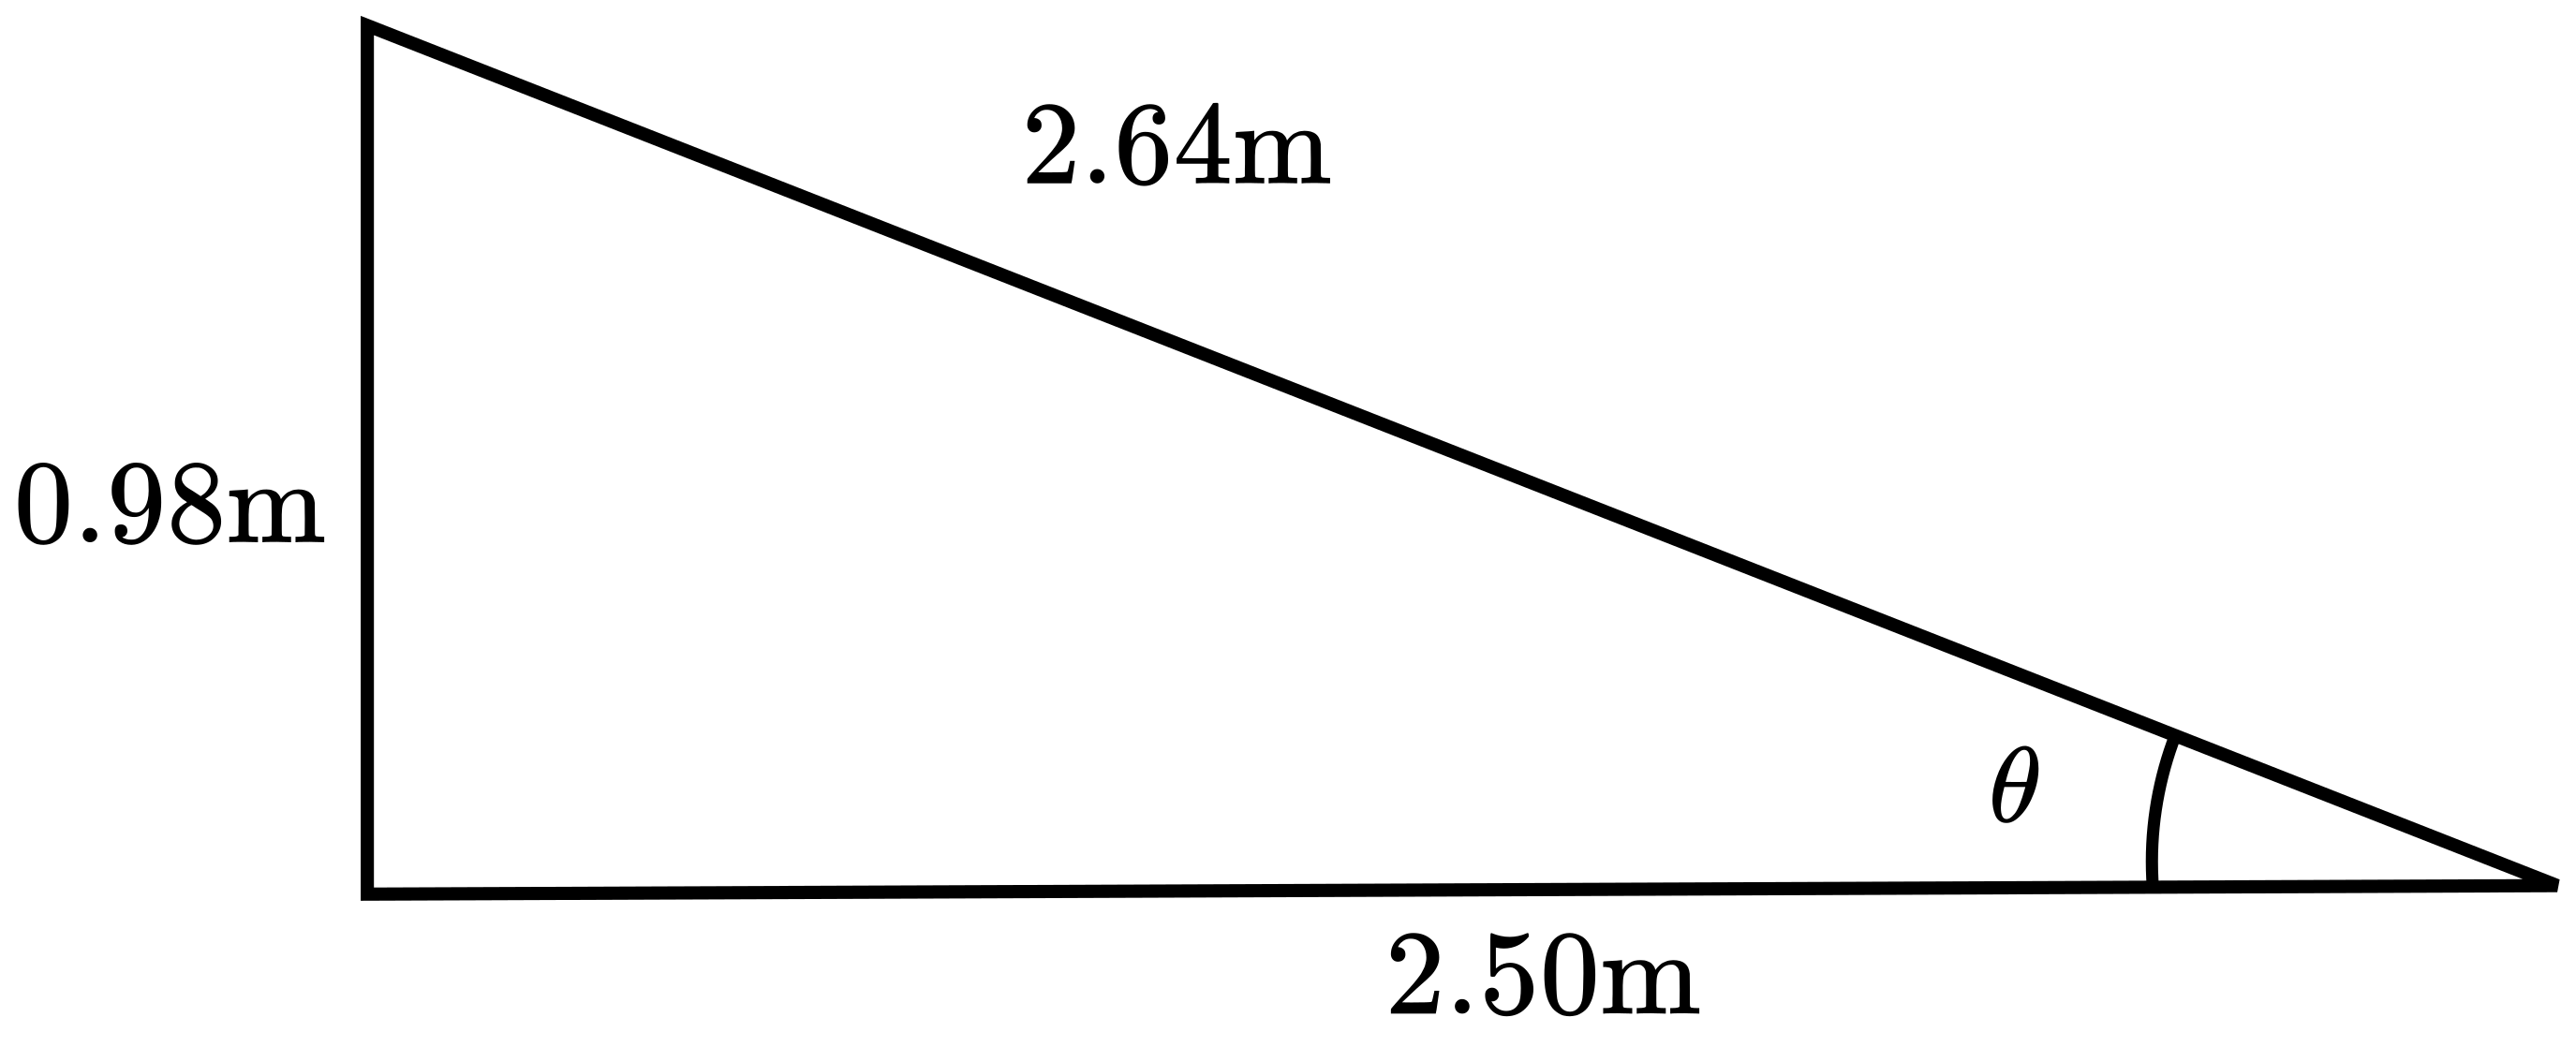
\includegraphics[width=0.35\paperwidth]{./Diagrams/LengthDiagram.png}
	\caption{Diagram showing the side lengths of triangle formed by incline plane}
\end{figure}


\subsubsection{Plotting}

\begin{figure}[H]
\centering
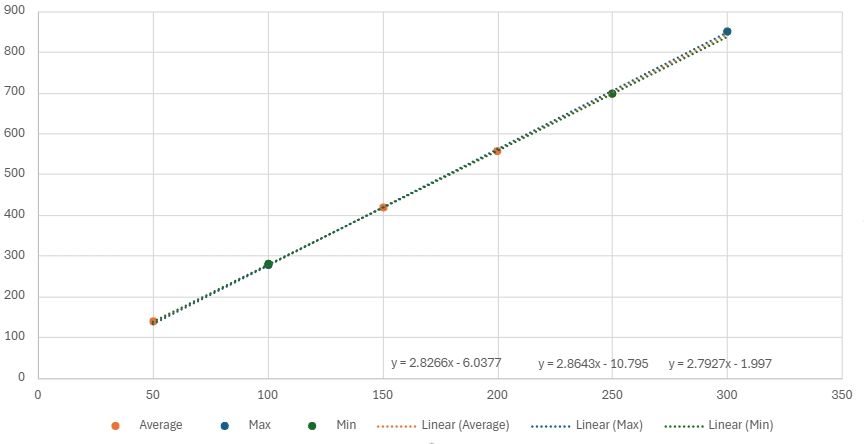
\includegraphics[width=0.8\paperwidth]{newresults.png}
\caption{Average $H_m$ ($x$-axis) and $C_m$ ($y$-axis) extrapolated from experimental data}
\end{figure}




\section{Discussion}
\subsection{Analysis of evidence}
\subsubsection{Identification of trends}
Figure 5 depicts a clear linear relationship formed by the data plotted. This supports the previously investigated relationship  $H_m=C_m\cdot{\sin(\theta)}$. However, clearly this graph represents the rearranged equation $C_m=H_m\cdot \frac{1}{{\sin(\theta)}}$.


This can be confirmed by determining the ratio between each of its points:
\\

As $H_m$ doubles from $50.14$ to $100.06$, $C_m$ increases by a factor of $\frac{278.05}{138.76}=2.0038\approx2.00$

As $H_m$ doubles from $278.05$ to $555.07$, $C_m$ increases by a factor of $\frac{555.07}{278.05}=1.9963\approx2.00$

\hfill

The presence of vertical shift in the line of best fit implies there is some inaccuracy in the data. In theory the relationship should be directly proportional
To find the angle, the gradient of the slope of average values for each trial can be extrapolated from the line of best fit, and substituted into the equation found for angle in terms of gradient.

\begin{align*}
\centering
\;\theta=&\;\sin^{-1}\left(\frac{1}{\textrm{gradient}}\right)\\
 =& \;\sin^{-1}\left(\frac{1}{2.8266}\right)\\
	=&\;20.7188^\circ
\end{align*}

\subsubsection{Uncertainty}

{\large \textbf{Finding uncertainty}\newline}
Since the value of $H_m$ was deliberately set, any uncertainty was due to the inherent random error in the scale used to measure it. By averaging $H_m$ across trials, a more reliable value can be found, however it should be noted that although this negates the effect of random error, the systematic uncertainty ($\pm0.005g$) is not affected as it is determined by the scale's precision. Therefore $H_m$ was assumed to be error free.

To find the absolute uncertainty in the gradient, the maximum and minimum slopes were required. By considering the two average carriage masses with the largest uncertainties, say $m_1, m_2$, then plotting the line between $m_1+\sigma_1$ and $m_2-\sigma_2$, then  $m_1-\sigma_1$ and $m_2+\sigma_2$, the equations of the maximum and minimum slopes could be solved as a line of best fit using Excel. This approach was chosen as when using the 'end points' of the data, the maximum slope found was smaller than the average.
\begin{center}
	\textbf{Absolute uncertainty in the gradient}
	\begin{align*}
		\centering
		\sigma(\textrm{gradient})=&\pm\frac{\textrm{max}-\textrm{min}}{2}\\
		\therefore\;\sigma(\textrm{gradient})=&\pm\frac{2.8643-2.7927}{2}\\
		=&\pm\frac{0.0716}{2}\\
		=&\pm0.0358
	\end{align*}
	
	\textbf{Absolute uncertainty in the angle}
	
	\begin{align*}
		\centering
		\sigma(\textrm{angle})=&\pm\frac{\textrm{max}-\textrm{min}}{2}\\
		\sigma(\textrm{angle})=&\pm\frac{\sin^{-1}(\frac{1}{2.8643})-\sin^{-1}(\frac{1}{2.7927})}{2}\\
		=&\pm0.274138198466^\circ 
	\end{align*}
	
\end{center}
\hfill

{\large \textbf{Possible sources of uncertainty}}



\textbf{Angle consistency}\newline
Since the experiment was conducted over multiple class periods, the experimental setup was dismantled and reassembled part way through. Additionally the plane was bumped on multiple occasions, requiring it to be returned back to its original location and angle. Despite the angle of the plane measuring the same throughout the experiment, the uncertainty in the tool used to set the angle of the plane ($\pm0.5^\circ$) meant that the angle was likely inconsistent. This was not accounted for in any way.

\textbf{Friction}\newline
It was assumed that the frictionless plane was completely frictionless. This was not the case, and multiple factors likely altered the degree of friction across it throughout the experiment.
It was noticed that when masses were in equilibrium, pushing the cart would cause it to move for a while, then slow down and stop. If the plane was truly frictionless then the plane would not have slowed down, but continued until it reached the end stop. It was theorised that the surface area of the carriage on the plane determined how much of an air pocket could form underneath it. This was briefly investigated as the type of carriage used was recorded for each trial. Considering one big carriage having the approximate equivalent surface area of two small carriages, the average uncertainty for each set of trials was plotted against the approximate carriage surface area. However, rather than a reduction in uncertainty as surface area increased, an increase was observed. 
Another source of friction is the pulley and string system that connects the masses. Although the pulley moves freely, there is likely play or static fiction in the system, as well as elasticity in the string.
\begin{figure}[h]
	\centering
	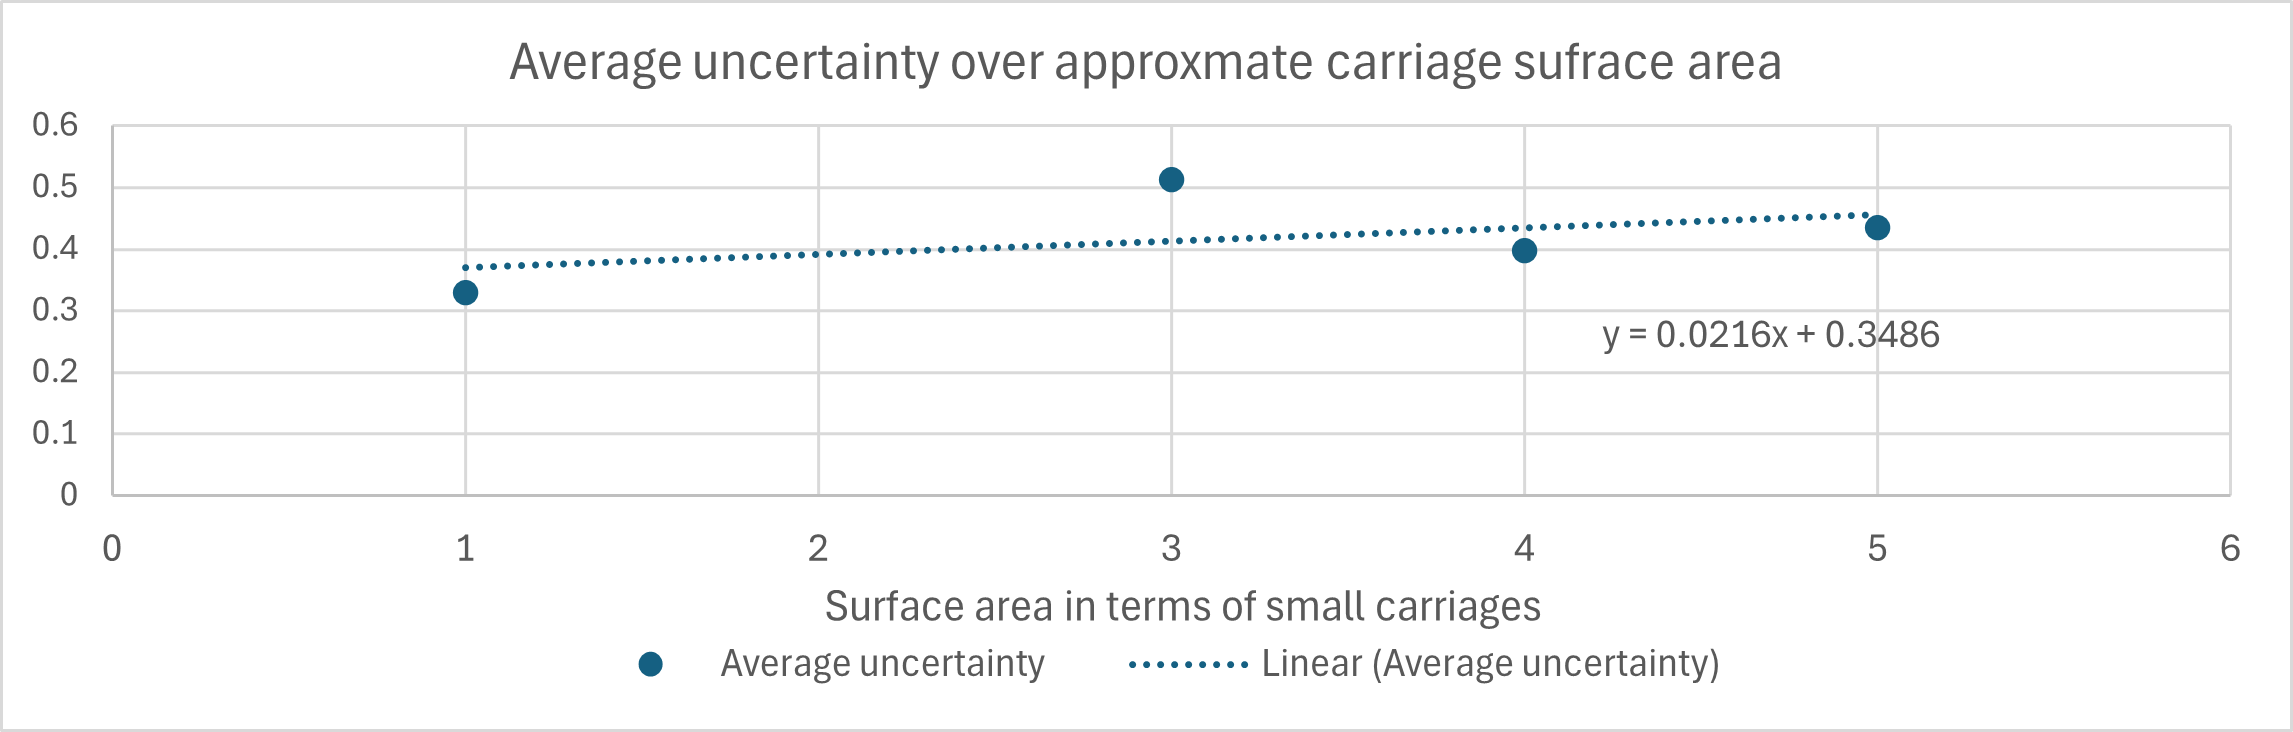
\includegraphics[width=0.7\paperwidth]{./images/ApproxCarriage.png}
	
\end{figure}


\section{Evaluation}

\subsection{Reliability and validity}


{	\large
	\textbf{Comparison to trigonometric calculations}}

Using the lengths of each side of the right angle triangle formed by the incline plane and the ground, the angle between them can be found. It was found that the angle differed based on which trigonometric function was used. 
 
 \begin{align*}
 	\sin^{-1}\left({\frac{0.98}{2.64}}\right)=&\;21.79^\circ\\
 	\cos^{-1}\left({\frac{2.50}{2.64}}\right)=&\;18.74^\circ\\
 	\tan^{-1}\left({\frac{0.98}{2.50}}\right)=&\;21.41^\circ\\
 \end{align*}
 
 This indicates error in the measurement process. While assuming these values are equally reliable, then averaging them, would give a valid angle, this process introduces uncertainty. It was decided that the most reliable values were the hypotenuse since it was the length of the incline plane and physically could not have changed, and the vertical measurement taken from the top of the plane to the ground, as it was the easiest to confirm as parallel during the measurement process.
 
 Considering the ruler only measured in half centimetre increments, its uncertainty was $\pm 0.25$cm, or $\pm0.0025$m. By considering the sine value of $\frac{2.64-\sigma}{0.98+\sigma}$, and $\frac{2.64+\sigma}{0.98-\sigma}$, the absolute uncertainty in this measurement can be found.
 \begin{align*}
 	 \sin^{-1}\left(\frac{0.98+0.0025}{2.64-0.0025}\right)=&\;21.87\\
 	 \sin^{-1}\left(\frac{0.98-0.0025}{2.64+0.0025}\right)=&\;21.71\\
 \end{align*}

 \begin{align*}
 	\sigma=&\;\frac{\textrm{max}-\textrm{min}}{2}
 	\\
 	=&\;\frac{21.87-21.71}{2}
 	\\
 	=&\;\pm0.08
 \end{align*}

 
 
 
 Therefore the angle of the slope as determined via trigonometry was $\sin\left({\frac{0.98}{2.64}}\right)=\;21.79^\circ \pm0.08$.
 


While the uncertainty is very low, this value is dissimilar to the angle obtained using the angle. If we consider $20^\circ$ or $21.79^\circ$ as the actual angle, we can find an approximate error of the angle found using masses.
\begin{center}
	\begin{large}
		
		\textbf{Assuming $\theta=21.79^\circ$}
	\end{large}
\end{center}

$$|\frac{20.72-21.79}{21.79}|=4.91\%$$
\begin{center}
	\begin{large}
		
		\textbf{Assuming $\theta=20.00^\circ$}
	\end{large}
\end{center}

$$|\frac{20.72-20}{20}|=3.60\%$$

These error values are generally considered low ($\geq5\%$), however it is unlikely that these values are reliable, due to poor procedure.

The possibility was considered that during the measurement process, the hypotenuse was measured as the length of the plane, rather than where the plane would intersect with the ground, to the point in which the string begins travelling downwards. Assuming $7$cm of unaccounted for length on either side of the plane, the total length of the hypotenuse would be $2.78$m. Assuming $10$cm of unaccounted for horizontal length due to poor procedure, the total length of the "Adjacent" side would be $2.60$m. These changes would result in an average angle across sine, cosine, and tangent calculations of $20.68^\circ \pm0.045^\circ$, which falls in line with the expected results.

\begin{figure}[H]
	\centering
	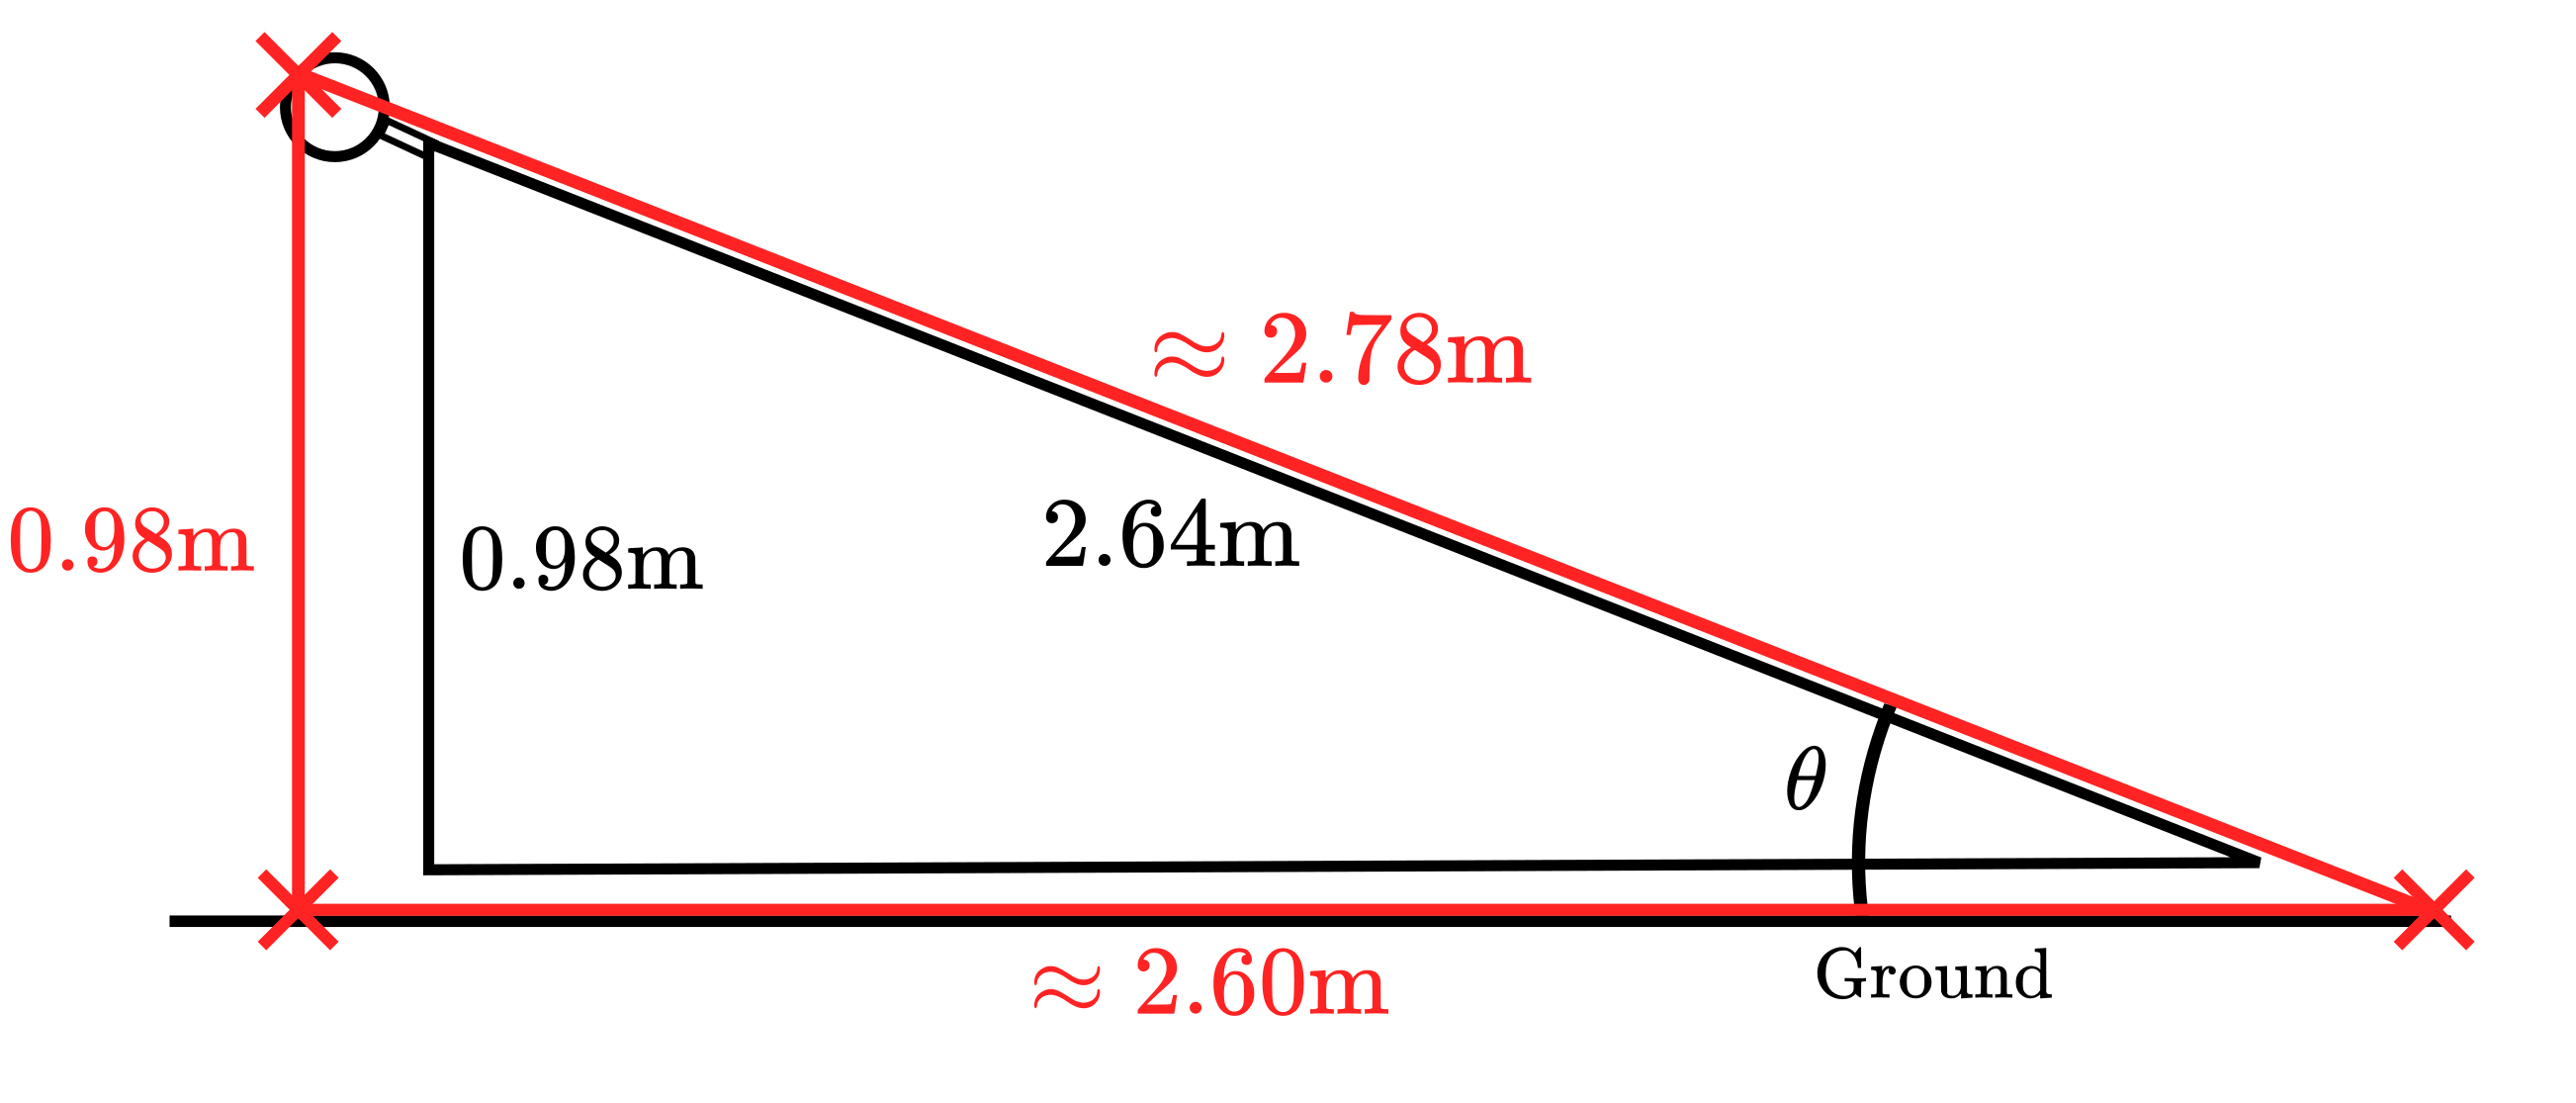
\includegraphics[width=0.5\paperwidth]{./Diagrams/LengthDiagramRevised.png}
	\caption{Recorded measurements (black) and theorised measurements (red)}
\end{figure}
However since these measurements are purely theoretical, they cannot be used to quantify error or any other results.




	{\large
	\textbf{Comparison to angle gun}}\\
As previously mentioned, the line of best fit constructed by the data did not cross through the origin, which implies error in the experimental process. This was likely due to the variables previously discussed, such as friction and procedural error. 
Considering the errors in the data derived from trigonometry, a reliable error analysis was unable to be conducted. The only option available is a direct comparison in terms of uncertainty and precision in comparison to the angle gun.
\begin{center}
	\textbf{Uncertainty comparison}
\end{center}

$$\sigma(\textrm{Angle gun})=\pm0.5^\circ>\sigma(\textrm{Mass method})=\pm{0.27^\circ}$$
Clearly the uncertainty of the angle found using masses in equilibrium is smaller than the uncertainty of the angle gun by nearly a factor of half. Additionally, the angle value obtained using masses has a greater precision of 2 decimal places, as opposed to none.

\subsection{Improvements and Extensions}

	{\large
	\textbf{Improvements}\\}

	The experimental process could be improved through the implementation of the following:
\begin{itemize}
	\item Conducting measurements using a rigid "square" (tool, not shape) to ensure that measurements are taken from the correct position and at angles parallel to the ground or other features. 
	\item A stronger blower fan could reduce friction, therefore improving accuracy. 
	\item More rigid string, or steel wire, could be utilised to remove the elastic component from the linkage between masses.
	\item A digital angle meter could be used to find the expected angle with more precision so that a reliable error analysis could be conducted.
\end{itemize}

	{\large
	\textbf{Extensions}}\\
The following extensions could extend data on a specific aspect of the experiment or pivot to investigation to a tangentially related topic.
\begin{itemize}
	\item A pivot to the investigation could investigate masses not in equilibrium and how their masses affect their acceleration. 
	\item Investigation into deceleration of masses when force is applied to quantify the friction of the supposedly "frictionless" plane.
	
\end{itemize}

\section{Conclusion}
This experiment quantified the angle of a frictionless plane using the relationship between a mass on the plane, and a hanging mass linked to it. Despite systematic and procedural errors such as friction, unintentional equipment reconfiguration, and incorrect measurementation, the angle was found with increased prevision and reduced uncertainty ($20.72^\circ \pm 0.27^\circ$) in comparison to conventional equipment, such as an angle gun ($20^\circ \pm 0.5^\circ$). It is evident that this is a viable method for determining angle when performed correctly, however, further investigation is required to determine the exact error of this method.



\newpage

\bibliography{./Bibliography/Physics_IA2.bib}

	
\end{document}